\section{Results}\label{sec:4-results}

\subsection{Hard Scattering}

The main \texttt{basic} example outputs a number of different files, assuming the main program was not modified. In particular, for either hard scattering or parton showering there are \texttt{.dat} files produced containing the kinematic variables for all of the events.

\begin{listing}[!ht]
\begin{minted}{text}
#cos(theta) rho         y           Q         x1
-0.951787   1.5357      0.498004    325.786   0.0229237	
-0.0794975  0.846551    0.0443711   87.5763   6.13877e-05	
-0.83998    1.21204     0.64568     114.893   0.0332578	
-0.138378   1.36989     0.107851    145.865   0.00029054	
-0.164968   0.418056    0.0662585   72.106    5.3322e-05	
-0.737887   0.668366    0.0813915   80.2655   7.61546e-05	
-0.4515     0.854714    0.667957    87.9612   0.0344976	
0.565371    0.49181     0.186333    74.3544   0.000198658	
-0.194654   0.830988    0.885909    86.8572   0.313566	
\end{minted}
\caption{The first ten lines of \texttt{events.dat}, the output file from the hard scattering simulation.}
\label{listing:events-dat}
\end{listing}

As an example, running the hard scattering simulation spits out a file titled \texttt{events.dat}, the first ten lines of which look like that given in Listing~\ref{listing:events-dat}. The variables, in order from left to right, are $\cos\theta$, the angle between the two final state particles, $\rho$, an intermediate calculational variable with no direct physical significance, $y$, the rapidity, a measure of the speed of the outgoing particles, $Q$, the center-of-mass energy of the process\footnote{This is not the center-of-mass energy of the proton-proton collision! Again, the subprocess involving the quarks occurs at a different energy related to the momentum fraction each quark carries.}, and $x_1$, the fraction of momentum of the proton the first quark carried.

\begin{figure}[ht]
  \centering
  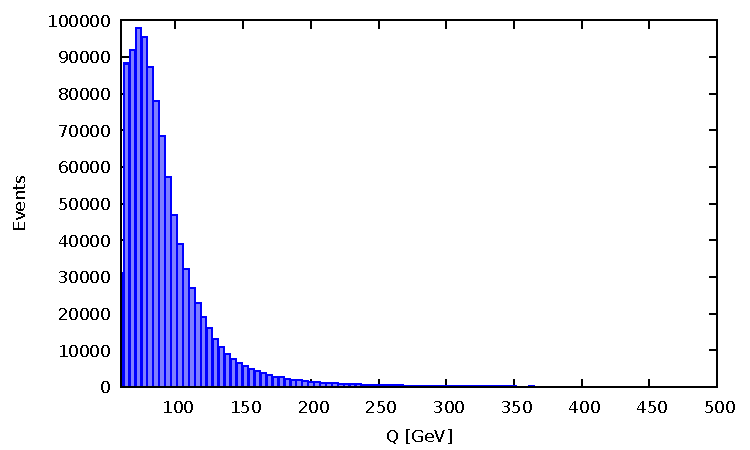
\includegraphics[width=0.4\linewidth]{./res/gfx/results/Q.pdf}
  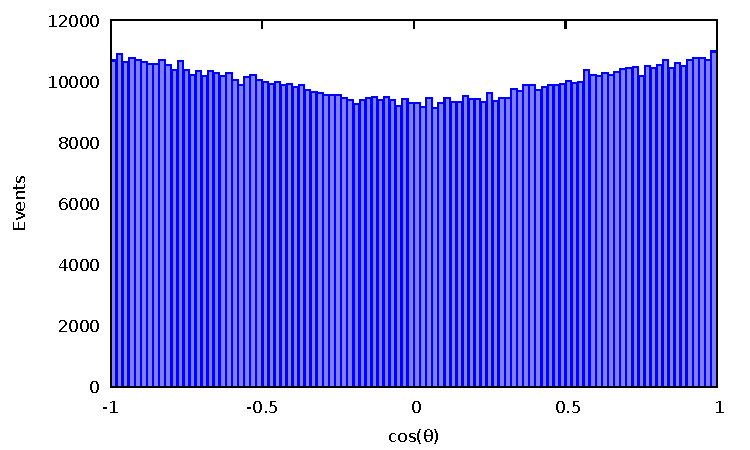
\includegraphics[width=0.4\linewidth]{./res/gfx/results/cos_theta.pdf}
  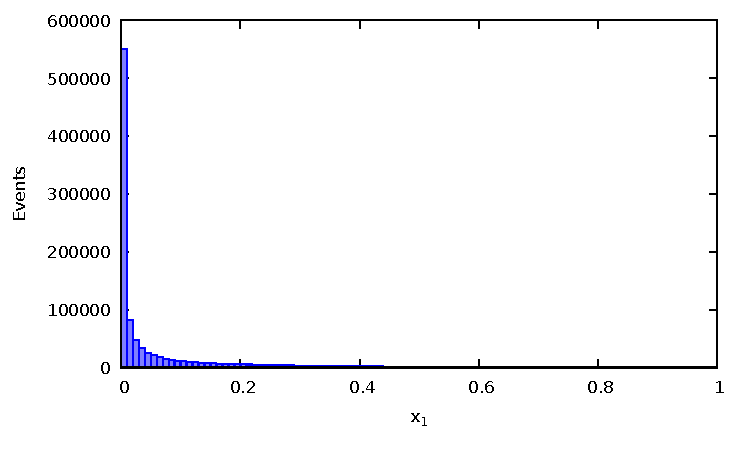
\includegraphics[width=0.4\linewidth]{./res/gfx/results/x1.pdf}
  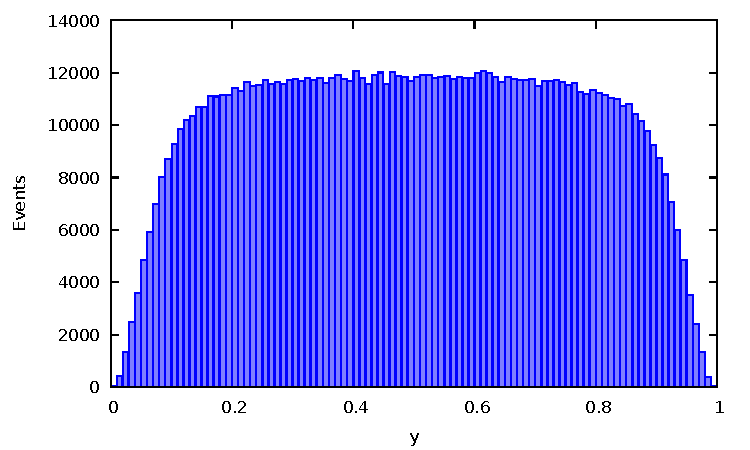
\includegraphics[width=0.4\linewidth]{./res/gfx/results/y.pdf}
  \caption{Outplot plots for distribution of the kinematic/phase space variables for the generated hard scattering events.}
  \label{fig:hard-scattering-dist}
\end{figure}

In Figure~\ref{fig:hard-scattering-dist} are distributions for all of these variables except for $\rho$, since it is an intermediate variable. It is important to note that all of these distributions make complete physical sense. First, the most easy to explain is the $\cos\theta$ distribution. It would make complete sense that scattering angles are possible; limits should instead start to pop up when looking at energies, rather than just the scattering angle. The $Q$ distribution tells us that lower energy events are significantly more likely than higher energy ones. This is not saying that the higher energy one goes the more likely lower energy events will show up, rather it is simply reflecting the fact that the phase space for the lower energy events gives a higher cross section. As we will see in the sensitivity and scenario analysis, as we increase the center-of-mass energy of the proton-proton collision,  this curve shifts to the right, reflecting the opposite of our naive assumption.

\begin{figure}[ht]
  \centering
  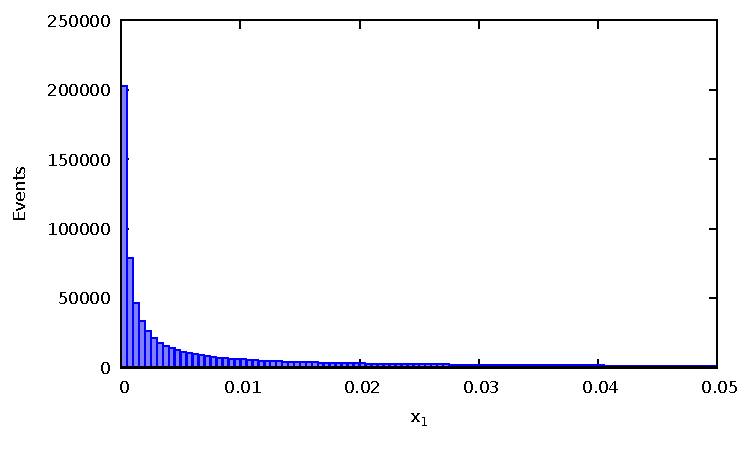
\includegraphics[width=0.75\linewidth]{./res/gfx/results/x1_new.pdf}
  \caption{$x_1$ distribution with modified $x$-limits to reflect its range.}
  \label{fig:x1-new}
\end{figure}

Additionally, in Figure~\ref{fig:x1-new} I have included another plot of the $x_1$ distribution to fully reflect the interesting fact that the majority of the events are with quarks that have a very small momentum fraction of the main proton. This is particularly interesting, but considering that, in the PDFs, there is a higher probability of finding quarks with lower momentum fractions, this checks out.

The rapidity distribution in Figure~\ref{fig:hard-scattering-dist} reflects similar physics. I mentioned before that rapidity was a measure of speed, which is true, but it is also a kind of measure of the angle between the particle and the beam axis, as well. The higher the rapidity, the faster the particle and the less of an angle it has against the beam axis. Therefore, based on the observation that the lower energy events have the higher probability for occuring at a particular center-of-mass energy, we would expect fewer of the super high speed and low angle events, which is exactly what we observe in the rapidity distribution. This also explains the slight dip for smaller scattering angles, as this would reflect particles with higher rapidity.


\subsection{Parton Showering}

\begin{listing}[!ht]
\begin{minted}{text}
#t      pT      m
31.1053 10.1835 17.7978	
14.6723 6.68227 9.90174	
25.9178 6.50954 12.9889	
18.2344 2.75489 7.08758	
18.2067 6.32354 10.7299	
22.1597 7.11254 12.5543	
18.3092 3.78753 8.32746	
25.3827 6.36348 12.7091	
20.8469 4.96856 10.1774	
\end{minted}
\caption{The first ten lines of 'emissions.dat,' the output data file for parton showering simulation.}
\label{listing:emissions-dat}
\end{listing}


Similarly, when running the parton showering part of the simulation, it spits out a file titled \texttt{emissions.dat}, the first ten lines of which look like Listing~\ref{listing:emissions-dat}. From left to right, the variables are $t$, the energy at which the emission occurred, $p_T$, the transverse momentum (perpendicular to the direction of the quark) of the quark and gluon, and the virtual mass of the quark and gluon. The virtual mass is interpreted as what the mass of a single particle with the same amount of energy traveling in same direction as the center-of-mass of the quark and gluon would be.

\begin{figure}[ht]
  \centering
  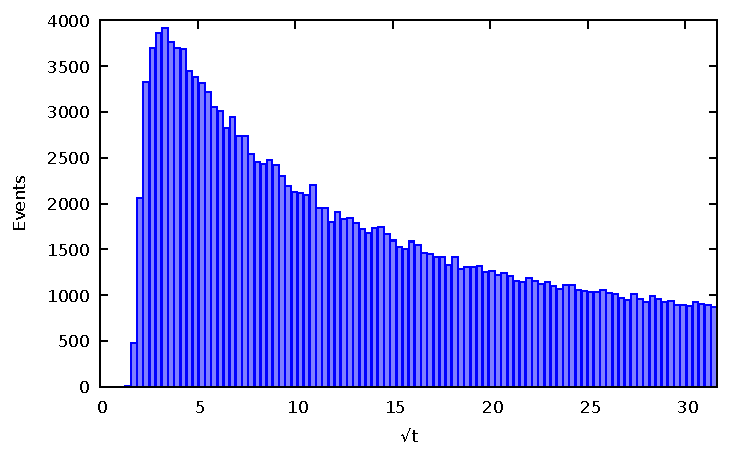
\includegraphics[width=0.32\linewidth]{./res/gfx/results/t.pdf}
  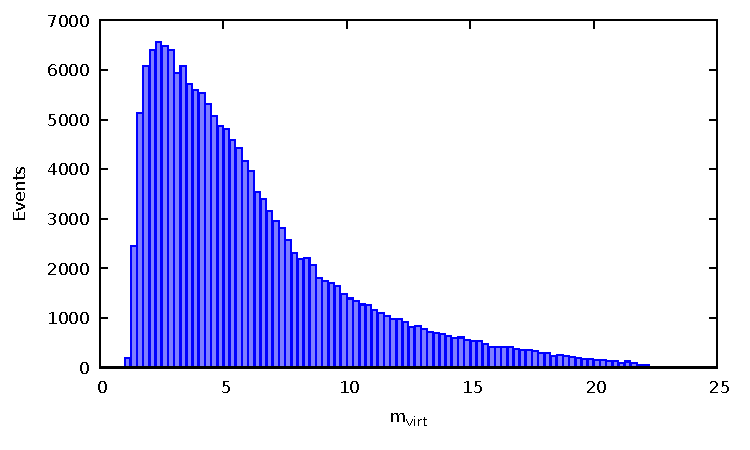
\includegraphics[width=0.32\linewidth]{./res/gfx/results/m.pdf}
  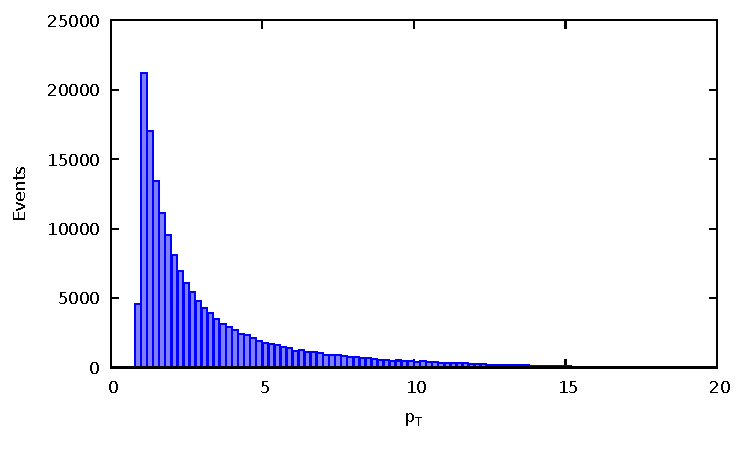
\includegraphics[width=0.32\linewidth]{./res/gfx/results/pT.pdf}
  \caption{Output plots for $t$, $m_{\mathrm{virt}}$, and $p_T$ for the generated parton showering events.}
  \label{fig:partonshower-dist}
\end{figure}

In Fig.~\ref{fig:partonshower-dist} are the generated plots for the $t$, $pT$, and $m_{\mathrm{virt}}$ distributions for the generated parton showering events. We notice that all the curves follow a roughly similar distribution and for the same reasons as the $Q$ distribution from the hard scattering case; that is, they peak at lower energies and fall off as the energy increases. This is most apparent in the $p_T$ plot. The $m_{\mathrm{virt}}$ plot has a less pronounced peak compared to the $p_T$ distribution, but this makes sense because this is taking into account the momenta of both the quark and the emitted gluon, whereas $p_T$ is in reference only to the emitted gluon. In the former, the emitted gluon is allowed to have a lower $p_T$, but if the quark still has a high energy, the virtual mass will remain higher. Of course, there is only so much energy to go around, so we still see it decrease in a similar manner, but the rounded peak is still expected.

Additionally, as a note, the $\sqrt{t}$ distribution is cutoff hard at $\qty[parse-numbers=false]{\sqrt{1000}}{\giga\electronvolt}$, because the initial evolution scale of the parton showering was $\qty{1000}{\giga\electronvolt}$ in the simulation runs for which these plots were generated. Further, in all of the plots, we are able to notice the impact of the evolution cutoff parameter, set at $\qty{1}{\giga\electronvolt}$ for these runs. The importance/sensitivity of this parameter is discussed further in the next section.


%%% Local Variables:
%%% mode: LaTeX
%%% TeX-master: "../../FinalMilestone"
%%% End:
